\section{Training}

\subsection{}

\begin{frame}
    \frametitle{Recap \& training objective}

    What we have so far
    \begin{itemize}
        \item<+-> A neural network $\f$
        \begin{itemize}
            \item User-selected \alert{architecture} (\# layers, \# neurons/layer, activations)
            \item Behavior set by thousands--billions of \alert{parameters} (weights \& biases) $\THETA = (\W_1, \b_1, \W_2, \b_2, \ldots)$
            \item \alert{Predicts} $\yh$ from $\x$ via $\yh = \f(\x; \THETA)$
            \item \alert{Universal approximation theorem}: $\f$ can model anything if $\THETA$ big enough
        \end{itemize}
        \item<+-> Gobs of \alert{data} pairs $\S = \{(\x, \y)\}$
        \item<+-> User-selected \alert{loss function} $L(\y, \yh)$
        \item<+-> Desire to minimize \alert{model risk} $R(\f; \THETA; \S) = \E_{(\x, \y) \in \S}(L(\y, \f(\x; \THETA)))$
    \end{itemize}

    \begin{block}{Training objective}<+->
        Iterate on $\THETA$ to minimize $R(\f; \THETA; \S)$
    \end{block}

    \begin{block}{Methodology}<+->
        Compute $\p{R}{\THETA}$ and use gradient descent
    \end{block}
\end{frame}

\begin{frame}
    \frametitle{Backpropagation}

    \uncover<+->{
        Since model risk $R$ is average over data of losses $L(\y, \f(\x; \THETA))$, gradient $\p{R}{\THETA}$ is average over data of $\p{L}{\THETA}$
    }

    \begin{block}{}<+->
        Backpropagation is how to compute $\p{L}{\THETA}$.
        It's literally just the chain rule.
    \end{block}

    \begin{itemize}
        \item<+-> Technique: symbolically pre-compute every element of $\p{L}{\THETA}$ via chain rule (one-time work)
        \begin{itemize}
            \item Software does this automatically
            \item Tedious, so we'll see one brief example next
        \end{itemize}
        \item<+-> When new datum $(\x, \y)$ arrives, plug in to get $\p{L}{\THETA}$
        \begin{itemize}
            \item Just multiplies, adds, \& activation functions---lightning fast
        \end{itemize}
        \item<+-> Average over data to get $\p{R}{\THETA}$
    \end{itemize}
\end{frame}

\begin{frame}
    \frametitle{Backpropagation example (1/3)}
    \begin{itemize}
        \item Single hidden-layer dense $\Reals^q \to \Reals^p$ neural network
        \item $n$ neurons with ReLU activation in hidden layer
        \item Mean squared error loss
    \end{itemize}
    \pause

    \begin{block}{}
        \vspace{-1em}
        \begin{align*}
            \hat{y}_k &= \sum_{j=1}^n v_{kj} \sigma\left(\sum_{i=1}^q w_{ji} x_i + b_j\right) + c_k,
            \quad
            k = 1, \ldots, p \\
            L(\y, \yh) &= \frac{1}{p} \sum_{k=1}^p (y_k - \hat{y}_k)^2
        \end{align*}
    \end{block}
    \pause

    Note: for ReLU $\sigma$, $\d{\sigma}{x} = H(x)$, the Heaviside step function

    \begin{equation*}
        \p{L}{\hat{y}_k} = \frac{2 (\hat{y}_k - y_k)}{p}
    \end{equation*}
\end{frame}

\begin{frame}
    \frametitle{Backpropagation example (2/3)}

    \begin{block}{}
        \vspace{-1em}
        \begin{align*}
            \hat{y}_k &= \sum_{j=1}^n v_{kj} \sigma\left(\sum_{i=1}^q w_{ji} x_i + b_j\right) + c_k,
            \quad
            k = 1, \ldots, p \\
            L(\y, \yh) &= \frac{1}{p} \sum_{k=1}^p (y_k - \hat{y}_k)^2, \qquad
            \p{L}{\hat{y}_k} = \frac{2 (\hat{y}_k - y_k)}{p}
        \end{align*}
    \end{block}
    \pause

    \begin{align*}
        \p{L}{v_{kj}} &= \p{L}{\hat{y}_k} \p{\hat{y}_k}{v_{kj}}
        = \frac{2 (\hat{y}_k - y_k)}{p} \sigma\left(\sum_{i=1}^q w_{ji} x_i + b_j\right) \\
        \pause
        \p{L}{c_k} &= \p{L}{\hat{y}_k} \p{\hat{y}_k}{c_k}
        = \frac{2 (\hat{y}_k - y_k)}{p}
    \end{align*}
\end{frame}

\begin{frame}
    \frametitle{Backpropagation example (3/3)}

    \begin{block}{}
        \vspace{-1em}
        \begin{align*}
            \hat{y}_k &= \sum_{j=1}^n v_{kj} \sigma\left(\sum_{i=1}^q w_{ji} x_i + b_j\right) + c_k,
            \quad
            k = 1, \ldots, p \\
            L(\y, \yh) &= \frac{1}{p} \sum_{k=1}^p (y_k - \hat{y}_k)^2, \qquad
            \p{L}{\hat{y}_k} = \frac{2 (\hat{y}_k - y_k)}{p}
        \end{align*}
    \end{block}
    \pause

    \begin{align*}
        \p{L}{w_{ji}} &= \sum_{k=1}^p \p{L}{\hat{y}_k} \p{\hat{y}_k}{w_{ji}}
        = \sum_{k=1}^p \frac{2 (\hat{y}_k - y_k)}{p} v_{kj} H\left(\sum_{i=1}^q w_{jl} x_l + b_j\right) x_i \\
        \pause
        \p{L}{b_j} &= \sum_{k=1}^p \p{L}{\hat{y}_k} \p{\hat{y}_k}{b_j}
        = \sum_{k=1}^p \frac{2 (\hat{y}_k - y_k)}{p} v_{kj} H\left(\sum_{i=1}^q w_{jl} x_l + b_j\right)
    \end{align*}

    \ldots You get the point.
\end{frame}

\begin{frame}[t]
    \frametitle{The trouble with gradient-based optimization}

    Gradient-based methods \citep{PressNR} seek local minima \\[1ex]

    The usual case:
    \begin{itemize}
        \item $\exists$ global minimization methods, but very slow
        \item Direct gradient descent usually bad
        \item Better methods: conjugate gradient, quasi-Newton
        \item \alert{Easily falls into non-global minima}
    \end{itemize}

    \begin{textblock}{6}(9, 11)
        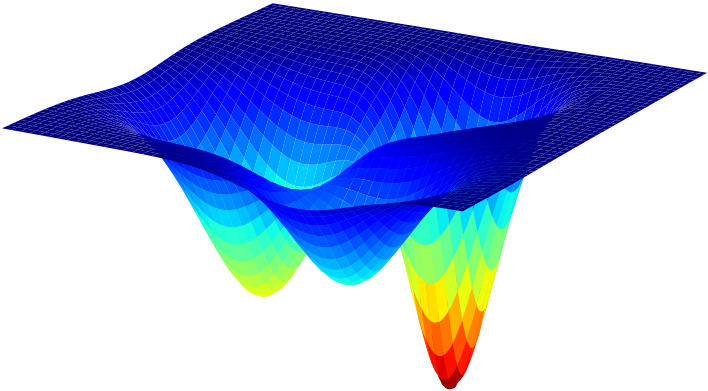
\includegraphics[width=\textwidth]{minima}
    \end{textblock}

    \pause

    For neural networks:
    \begin{itemize}
        \item Given data set $\S = \{(\x_i, \y_i)\}$ with enormous $|\S|$
        \item Want to find $\THETA$ to minimize approximate model risk $\displaystyle R(\f; \THETA; \S) = \frac{1}{|\S|} \sum_{(\x, \y) \in \S} L(\y, \f(\x; \THETA))$
        \item \alert{Intractable}
    \end{itemize}
\end{frame}

\begin{frame}
    \frametitle{Stochastic gradient descent \& mini-batching}
    \begin{algorithmic}[1]
        \uncover<+->{\FOR{$\text{epoch} = 1, \ldots, n_\text{epochs}$}}
        \uncover<+->{\STATE Randomize the data order of $\S$}
        \uncover<+->{\WHILE{not done with $\S$}}
        \uncover<+->{\STATE Peel off the next $k \ll |\S|$ elements of $\S$ into the \alert{mini-batch} $\M$}
        \uncover<+->{
            \STATE \label{item:gradient}
            Compute $\h = \p{R(\f; \THETA; \M)}{\THETA}$ using only the mini-batch $\M$
        }
        \uncover<+->{
            \STATE Take a small step against the gradient: $\THETA \leftarrow \THETA - \alpha\h$ with $0 < \alpha \ll 1$
        }
        \uncover<3->{\ENDWHILE}
        \ENDFOR
    \end{algorithmic}
    \vspace{1ex}

    \uncover<+->{Terminology:}
    \begin{itemize}[<.->]
        \item \alert{Learning rate}: $\alpha$
        \item \alert{Mini-batch size}: $k = |\M|$ (often just called \emph{batch size})
        \item \alert{Iteration}: a single gradient update
        \item \alert{Epoch}: a complete pass through the data
    \end{itemize}
\end{frame}

\begin{frame}
    \frametitle{Why stochastic gradient descent \& mini-batching?}
    It kills two birds with one stone

    \begin{block}{Tractability}
        \textcolor{red}{Gradient descent}: intractable to compute gradient $\p{R(\f; \THETA; \S)}{\THETA}$ when $|\S| \approx \dim(\THETA) = \O(10^3 \text{--} 10^{10})$ \\[1ex]
        \textcolor{blue}{SGD}: $\p{R(\f; \THETA; \M)}{\THETA}$ tractable when $|\M| = \O(10^1 \text{--} 10^3)$
    \end{block}

    \begin{block}{Global minimization}
        \textcolor{red}{Gradient descent}: easily falls into local minima \\[1ex]
        \textcolor{blue}{SGD}: stochastic because it takes gradient steps based on random small mini-batches
        \begin{itemize}
            \item Over long-run average, SGD mimics true gradient using all data
            \item In short-run, stochasticity gives SGD a chance to climb out of local minima if needed
        \end{itemize}
    \end{block}
\end{frame}

\begin{frame}
    \frametitle{SGD-based optimizers}
    \uncover<+->{Issues with vanilla SGD}
    \begin{itemize}
        \item In $\Reals^n$ with $n \gg 1$, most critical points are saddle points
        \item SGD easily gets stuck in saddle points
        \item In gradient step $\THETA \leftarrow \THETA - \alpha \bnabla R$, need to decay learning rate $\alpha$
    \end{itemize}

    \uncover<+->{Better alternatives}
    \begin{itemize}[<+->]
        \item<.-> Momentum: $\THETA \leftarrow \THETA - \alpha \bnabla R + \eta \mathbf{\Delta}\THETA$---encourages continuing previous update \citep{RumelhartNature86}
        \item RMSprop: divide learning rate by mean of recent gradient norms \citep{TielemanRMSProp}
        \item Adagrad: each parameter has own learning rate determined by its gradients \citep{DuchJMLR11}
        \item Adadelta: improves Adagrad by making learning rate decay less aggressive \citep{Zeiler12}
        \item \alert<+->{Adam}: adaptive learning rate \& momentum \citep{KingmaICLR15}
    \end{itemize}

    \uncover<.->{Short: use Adam; it's generally best and works great out-of-the-box}
\end{frame}

\begin{frame}
    \frametitle{Mini-batch size}

    Mini-batch size not a random decision; can have huge effects on training
    \begin{itemize}
        \item Mini-batch size usually integer power of 2---better GPU optimization
        \item $\text{Stochasticity} \sim \dfrac{\text{learning rate}}{(\text{mini-batch size}) (1 - \text{momentum})}$ \citep{SmithNIPS17}
        \item Historically, $\text{size} = 16 \text{--} 256$ common
        \item Growing trend toward extremely large (e.g., 8,192+) sizes
    \end{itemize}
    \pause

    Choosing mini-batch size
    \begin{itemize}
        \item Smaller: more stochastic
        \begin{itemize}
            \item Better at escaping non-global minima
        \end{itemize}
        \item Larger: less stochastic
        \begin{itemize}
            \item Better at converging to deep, narrow minima
            \item Faster---better GPU optimization
            \item But limited by available GPU memory
        \end{itemize}
    \end{itemize}
\end{frame}

% Initialization
% Powers of 2.
% Local/global minima
% Including train/validation/test, or put in separate section.
% Under/overfit

%%% Local Variables:
%%% mode: latex
%%% TeX-master: "../nn"
%%% End:
